\documentclass{article}
\usepackage[utf8]{inputenc}
\usepackage{graphicx}
\usepackage{fancyhdr}
\usepackage{verbatim}
\pagestyle{fancyplain}
\author{Mikkel Kragh Mathiesen, Jannik Gram, Rune \& Rasmus Abrahams{\tt (son|en)}}
\title{Oplæg 2: Design af eksperimenter}
\date{\today}
\lhead{Mikkel, Jannik, Rune \& Rasmus}
\rhead{\today}
\begin{document}

\maketitle

\tableofcontents

\newpage

\section{Indledning}
Nu til dags er båndbredden over netværk højere end båndbredden til en lokal harddisk --- eller er den? Vi vil udføre et eksperiment for at se, om udsagnet er sandt.

% 1
\section{Eksperimentdesign}

% 1.a
\subsection{Tidsmåling}
\textit{Tid måles med et ur}; I forsøget vil tiden blive målt med biblioteket {\tt Time::HiRes} i Perl. Tiden måles fra lige før filens overførsel starter og slutter lige efter. Her kan opstå problemer med buffering, da det er muligt at filen ikke er blevet skrevet færdig, når kopieringen terminerer.

% 1.b
\subsection{Tilgangsmønster for disk}
I eksperimentet bliver der antaget, at data læses sekventielt fra disken. Dette er imidlertid ikke realistisk, da der oftest læses mange tilfældige steder på disken samtidigt. Det burde dog ikke have den store effekt på resultaterne af eksperimentet, da der i begge forsøg benyttes harddiske, som man må antage opfører sig nogenlunde ens.

% 1.c
\subsection{Andre Parametre}
\subsubsection{Caching}
I alle moderne operativsystemer opererer filsystemet med en cache, således at en del af maskinens ellers ubenyttede RAM benyttes til at gemme de senest læste filer. Hvis den samme fil læses mange gange, vil det derfor kun generere diskaktivitet første gang --- medmindre filen er meget stor, en stor del af den fysiske RAM bruges af kørende programmer eller tilstrækkelig mange filer åbnes i mellemtiden.

Netop dette er den tekniske begrundelse for, at vi har valgt at ændre eksperimentet til at teste skrivninger, da disse af gode grunde ikke kan caches. Læsningen af den fil, der skal skrives, bliver derimod cachet forudsat, at der foretages en dummy-læsning inden eksperimentet startes --- dermed sikres det at flytning af en fil lokalt kun fremprovokerer en skrivning og ikke en læsning.

\subsubsection{Filsystem}
Det er også vigtigt hvilket filsystem, der bruges på de forskellige diske, der indgår i forsøget. Som et ekstremt eksempel vil tmpfs slet ikke bruge disken, men vores primære problemer vil forventeligvis være med netværksfilsystemer. For eksempel vil sshfs være tungt grundet kryptering, mens nfs, samba og lignende benytter en meget gammel og ineffektiv protokol.

\subsubsection{CPU som flaskehals}
Ved overførsel over netværk kan CPU'en virke som flaskehals. For eksempel bruger {\tt sshfs} CPU-intensiv kryptering, som kan begrænse hastigheden af overførslen.

\subsubsection{Hardware}
Harddiske, netværkskort, bundkort og CPU er alle en faktor, som kan have noget at sige for hastighederne.

\subsubsection{Netværksbelastning}
Belastning på netværket vil formindske båndbredden på det givne tidspunkt og derved forværre den eksterne disks overførselstider.

\subsubsection{Andre processor/forstyrrelser}
Moderne operativsystemer er hele tiden i gang med ting i baggrunden som for eksempel løbende defragmentering. Alt dette er med til at lave støj i resultaterne.

% 1.d
\subsection{Tese}
Båndbredden over netværk er langt højere end båndbredden til en harddisk så hvis man skriver tilstrækkeligt store filer til en disk vil der ikke være forskel på skrivehastigheden mellem en netværksforbundet og en lokal harddisk. Bemærk dog at der vil blive målt skrivninger og ikke læsninger.

% 2
\section{Implementering}

% 2.a
\subsection{Omstændigheder}

Et Perl-script (se figur \ref{kode}) genererer filer af størrelser fra 5 MB til 120 MB med 5 MB intervaller. Hver fil overføres til destinationen 8 gange, hvorefter gennemsnittet for overførslerne bliver beregnet. Dette bliver gjort både lokalt på en computer og til en harddisk på en computer på netværket. De overførte filer består af tilfældigt indhold af de angivne størrelser. Testen over netværk bliver gjort med netværkskabel frem for trådløst netværk for at mindste latenstid, tabte pakker og så videre. Derudover vil netværksdisken blive monteret ved hjælp af Samba.

\begin{figure}
	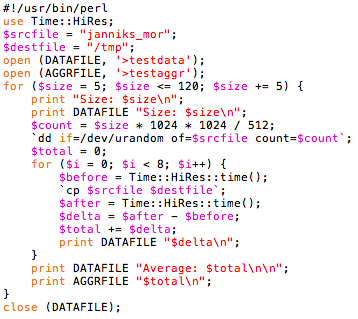
\includegraphics[width=4in]{kode.png}
	\caption{Perl-scriptet}
	\label{kode}
\end{figure}

% 2.b
\subsection{Graf}
På figur \ref{ploto} ses en graf for, hvor lang tid filerne af forskellige størrelser tager at overføre på henholdsvis en netværksdisk og en lokal disk. Umiddelbart tager det dobbelt så lang tid at overføre over netværk hele vejen igennem. Forholdet mellem lokal og netværk kan ses på figur \ref{plotforhold}, som også viser at overførsel over netværk er omkring 2 gange så langsomt. Forholdet udvikler sig rimelig lineært.

\begin{figure}
	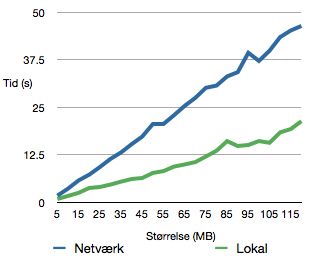
\includegraphics[width=4in]{ploto.png}
	\caption{Hastigheden for lokal og netværk.}
	\label{ploto}
\end{figure}

\begin{figure}
	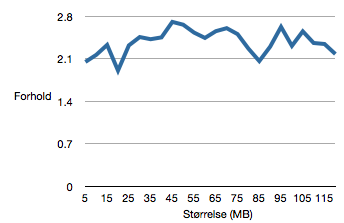
\includegraphics[width=4in]{plotforhold.png}
	\caption{Forholdet mellem de to hastigheder.}
	\label{plotforhold}
\end{figure}

% 2.c
\subsection{Teseoverlevelse}
Under antagelse af, at eksperimentet er fornuftigt udført, er konklusionen, at tesen er blevet succesfuldt falsificeret og dermed afvist, da forholdet mellem lokal- og netværksforbundet disk tendenserer til at være konstant. Det er svært tænkeligt, at endnu større filer vil ændre på dette, da netværksaktivitet alligevel bliver brudt op i pakker, der sendes hver for sig.

Antagelsen om eksperimentets holdbarhed er dog ikke helt berettiget. Der er en del usikkerhed, hvoraf kun en delmængde er blevet taget hånd om. Derfor vil det give god mening at undersøge, om uønskede faktorer fremprovokerede et falsk negativ. De mest umiddelbare tiltag er at bruge et netværksfilsystem af nyere dato og at finjustere blokstørrelsen til kopiering.

% 3
\section{Ræssonnement}

% 3.a
\subsection{Afstand}
Forøget afstand mellem disk og maskine har flere konsekvenser. Jo længere afstand, des større sandsynlighed for at en sendt pakke bliver tabt undervejs. Derudover bliver latenstiden højere, hvilket kombineret med det tidligere gør at båndbredden bliver meget lavere.

% 3.b
\subsection{Netværksudstyr}
Netværksudstyr, som router og firewall, er alt sammen med til at tilføje yderligere kompleksitet og forsinkelse.

% 3.c
\subsection{Samba}
I mellemtiden har vi fundet ud af, at Samba ikke er særligt optimal til filoverførsel. Dette har været med til at vise, at en overførsel over netværk er meget langsommere end en lokal overførsel.

\section{Perspektivering i forhold til artikler}

Stewart er netop frustreret over en mangel på sådan rigid opstillelse af teser og be- eller akræftning af disse. Han ville derfor formentlig acceptere vores grundlæggende metode og kalde det \textit{computer science}, omend vores udførsel og faktiske planlægning af eksperimentet efterlader noget at ønske. Han synes at gå ind for Poppers forudsætninger for videnskab, som kræver formelle og falsificerbare teser og rig mulighed for ekstern afprøvning/bekræftelse. Vores eksperiment er i teorien replikerbart, men i praksis er det ikke tilnærmelsesvist grundigt nok dokumenteret: det brugte hardware er ikke specificeret, og eksempelvis netværk har en masse usikkerhed, der ikke er taget højde for.   

\end{document}
